
%(BEGIN_QUESTION)
% Copyright 2011, Tony R. Kuphaldt, released under the Creative Commons Attribution License (v 1.0)
% This means you may do almost anything with this work of mine, so long as you give me proper credit

Create a computer spreadsheet to calculate the width of the {\it Fresnel zone} between two antennas given frequency, path distance, position from one antenna, and Fresnel zone number.  A sample layout is presented here, where yellow shading represents values to enter, and blue shading represents values calculated by the spreadsheet:

$$\includegraphics[width=15.5cm]{i00332x01.eps}$$

\vskip 20pt \vbox{\hrule \hbox{\strut \vrule{} {\bf Suggestions for Socratic discussion} \vrule} \hrule}

\begin{itemize}
\item{} Explain how you may {\it test} your finished spreadsheet program to see that it correctly calculates the Fresnel zone widths. 
\item{} If we are concerned with the Fresnel zone clearing a space between two parallel trees to either side of the line-of-sight, do we need to calculate {\it radius} or {\it diameter}?
\item{} If we are concerned with the Fresnel zone clearing the ground, do we need to calculate {\it radius} or {\it diameter}?
\end{itemize}

\underbar{file i00332}
%(END_QUESTION)





%(BEGIN_ANSWER)


%(END_ANSWER)





%(BEGIN_NOTES)


%INDEX% Computer spreadsheet exercise: Fresnel zone width calculator
%INDEX% Electronics review, Fresnel zones for radio links

%(END_NOTES)


